\documentclass[a4paper,10pt,twocolumn]{article}
\usepackage[english]{babel}
\usepackage[style=ieee,backend=bibtex]{biblatex} \bibliography{ref.bib}
\usepackage[hidelinks]{hyperref}
\usepackage{fancyhdr}
\usepackage{float}
\usepackage{graphicx}
\usepackage[latin1]{inputenc}
\usepackage{nomencl}
\usepackage{multicol}
\usepackage{siunitx}
\usepackage{tikz}
    \usetikzlibrary{arrows}
    \usetikzlibrary{patterns}
    \usetikzlibrary{3d}
\usepackage{titling}
\usepackage{xspace}

\newcommand{\Comsol}{\textsc{Comsol}\xspace}
\newcommand{\comsol}{\textsc{comsol}\xspace}
\newcommand{\Cmos}{\textsc{Cmos}\xspace}
\newcommand{\cmos}{\textsc{cmos}\xspace}
\newcommand{\Mems}{\textsc{Mems}\xspace}
\newcommand{\mems}{\textsc{mems}\xspace}

% Top matter
\title{\Mems Multimorph Temperature Sensors in
    \Comsol~Multiphysics\textsuperscript{\textregistered}}
\author{Z0966990}
\date{\today}

% Headers and footers
\pagestyle{fancy}
\fancyhf{}
\lhead{\includegraphics[width=0.1\textwidth]{img/Durham.png}}
\chead{\thetitle}
\rhead{\theauthor}
\cfoot{\thepage}

\begin{document}

% Title and abstract
\thispagestyle{plain}

\twocolumn[{
\begin{@twocolumnfalse} \centering
    \includegraphics[width=0.2\textwidth]{img/Durham.png}\\
    \Large\thetitle
    \vskip0.2em
    \large Level 3 Semiconductor, Physics and Devices\\
    \vskip0.4em
    \large\theauthor\\
    \vskip0.4em
    \large\thedate\\
    \hrulefill
    \renewcommand{\abstractname}{\large Abstract}
    \begin{abstract}
        In this report it is detailed how
    \end{abstract}
    \vskip\parsep
\end{@twocolumnfalse}
}]


\makenomenclature

% Acronyms
\nomenclature[A0]{\mems}{Microelectromechanical systems}

\printnomenclature

\begin{figure}[h]
    \centering
    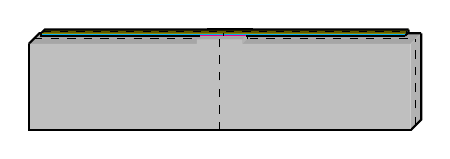
\begin{tikzpicture}[scale=0.4\textwidth/0.840cm]
        % Substrate
        \begin{scope}[canvas is zx plane at y=0.190]
            \path [fill=lightgray!140] (0,0) rectangle (0.060,0.840);
            \draw [thin,dashed] (0.060/2,0.000) -- (0.060/2,0.840);
            \draw [thick] (0.060,0.000) -- (0.000,0.000) -- (0.000,0.840);
        \end{scope}
        \begin{scope}[canvas is zx plane at y=0.200]
            \path [fill=lightgray!140] (0.000,0.370) rectangle (0.060,0.470);
            \draw [thin,dashed] (0.000,0.840/2) -- (0.060,0.840/2);
            \draw [thick] (0.000,0.370) -- (0.000,0.470);
        \end{scope}
        \begin{scope}[canvas is yz plane at x=0.470]
            \path [fill=lightgray!120] (0.190,0.000) rectangle (0.200,0.060);
            \draw [thin,dashed] (0.190,0.060/2) -- (0.200,0.060/2);
            \draw [thick] (0.190,0.000) -- (0.200,0.000);
        \end{scope}
        \begin{scope}[canvas is yz plane at x=0.840]
            \path [fill=lightgray!120] (0,0) rectangle (0.190,0.060);
            \draw [thin,dashed] (0.000,0.060/2) -- (0.190,0.060/2);
            \draw [thick] (0.190,0.000) -- (0.000,0.000) -- (0.000,0.060);
        \end{scope}
        \begin{scope}[canvas is xy plane at z=0.060]
            \path [fill=lightgray] (0.000,0.000) -- (0.840,0.000) -- 
                (0.840,0.190) -- (0.470,0.190) -- (0.470,0.200) --
                (0.370,0.200) -- (0.370,0.190) -- (0.000,0.190) --
                (0.000,0.000);
            \draw [thin,dashed] (0.840/2,0.000) -- (0.840/2,0.200);
            \draw [thick] (0.840,0.000) -- (0.000,0.000) -- (0.000,0.190);
        \end{scope}

        % Layers faces
        \begin{scope}[canvas is zx plane at y=0.206]
            \path [fill=olive!140] (0.020,0.020) rectangle (0.040,0.820);
            \draw [thin,dashed] (0.060/2,0.020) -- (0.060/2,0.820);
            \draw [thick] (0.040,0.020) -- (0.020,0.020) -- (0.020,0.820);
        \end{scope}
        \begin{scope}[canvas is yz plane at x=0.820]
            \path [fill=olive!120] (0.204,0.020) rectangle (0.206,0.040);
            \path [fill=cyan!120] (0.202,0.020) rectangle (0.204,0.040);
            \path [fill=magenta!120] (0.200,0.020) rectangle (0.202,0.040);
            \draw [thin,dashed] (0.200,0.060/2) -- (0.206,0.060/2);
            \draw [thick] (0.206,0.020) -- (0.200,0.020) -- (0.200,0.040);
        \end{scope}
        \begin{scope}[canvas is xy plane at z=0.040]
            \path [fill=olive] (0.020,0.204) rectangle (0.820,0.206);
            \path [fill=cyan] (0.020,0.202) rectangle (0.820,0.204);
            \path [fill=magenta] (0.020,0.200) rectangle (0.820,0.202);
            \draw [thin,dashed] (0.840/2,0.200) -- (0.840/2,0.206);
            \draw [thick] (0.820,0.200) -- (0.470,0.200);
            \draw [thick] (0.370,0.200) -- (0.020,0.200) -- (0.020,0.206);
        \end{scope}



    \end{tikzpicture}
\end{figure}

\begin{figure}[h]
    \centering
    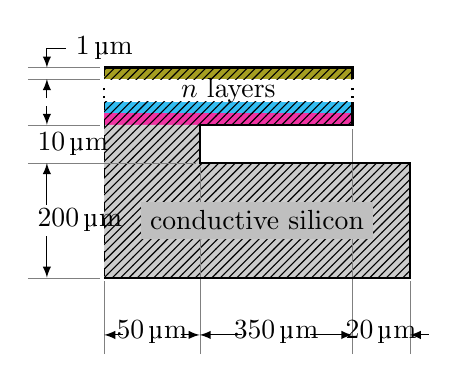
\begin{tikzpicture}[scale=0.4\textwidth/1cm]
        % Layers
        \path [fill=olive!80]   (0.20,0.72) rectangle (0.85,0.75);
        \path [fill=cyan!80]    (0.20,0.63) rectangle (0.85,0.66);
        \path [fill=magenta!80] (0.20,0.60) rectangle (0.85,0.63);
        \path [fill=lightgray!80] (0.20,0.20) -- (1.00,0.20) -- (1.00,0.50) -- 
            (0.45,0.50) -- (0.45,0.60) -- (0.20,0.60) -- (0.20,0.20);
        \path [pattern=north east lines] (0.20,0.72) rectangle (0.85,0.75);
        \path [pattern=north east lines] (0.20,0.63) rectangle (0.85,0.66);
        \path [pattern=north east lines] (0.20,0.60) rectangle (0.85,0.63);
        \path [pattern=north east lines] (0.20,0.20) -- (1.00,0.20) --  
            (1.00,0.50) -- (0.45,0.50) -- (0.45,0.60) -- (0.20,0.60) --
            (0.20,0.20);
        
        % Witness lines
        \draw [gray,ultra thin] (0.00,0.75) -- (0.19,0.75);
        \draw [gray,ultra thin] (0.00,0.72) -- (0.19,0.72);
        \draw [gray,ultra thin] (0.00,0.60) -- (0.19,0.60);
        \draw [gray,ultra thin] (0.00,0.50) -- (0.44,0.50);
        \draw [gray,ultra thin] (0.00,0.20) -- (0.19,0.20);

        \draw [gray,ultra thin] (0.20,0.00) -- (0.20,0.19);
        \draw [gray,ultra thin] (0.45,0.00) -- (0.45,0.49);
        \draw [gray,ultra thin] (0.85,0.00) -- (0.85,0.59);
        \draw [gray,ultra thin] (1.00,0.00) -- (1.00,0.19);

        % Outline
        \draw [thick] (0.20,0.20) -- (1.00,0.20) -- (1.00,0.50) -- (0.45,0.50)
            -- (0.45,0.60) -- (0.85,0.60) -- (0.85,0.66);
        \draw [dotted,thick] (0.85,0.67) -- (0.85,0.71);
        \draw [thick] (0.85,0.72) -- (0.85,0.75) -- (0.20,0.75);
        \draw [dashed] (0.20,0.75) -- (0.20,0.72);
        \draw [dotted,thick] (0.20,0.67) -- (0.20,0.71);
        \draw [dashed] (0.20,0.66) -- (0.20,0.20);

        % Labels
        \node at (0.525,0.69) {$n$ layers};
        \node [align=center,fill=lightgray] at (0.60,0.35) {conductive silicon};

        % Dimensions
        \node [right] at (0.10,0.80) {\SI{1}{\micro\meter}};
        \draw [latex-] (0.05,0.75) -- (0.05,0.80) -- (0.10,0.80);
        \draw [-latex] (0.05,0.67) -- (0.05,0.72);
        \draw [latex-] (0.05,0.60) -- (0.05,0.65);
        \node [right] at (0.00,0.55) {\SI{10}{\micro\meter}};
        \draw [-latex] (0.05,0.39) -- (0.05,0.50);
        \node [right] at (0.00,0.35) {\SI{200}{\micro\meter}};
        \draw [latex-] (0.05,0.20) -- (0.05,0.31);

        \draw [latex-] (0.20,0.05) -- (0.25,0.05);
        \node [above] at (0.325,0.00) {\SI{50}{\micro\meter}};
        \draw [-latex] (0.40,0.05) -- (0.45,0.05);
        \draw [latex-] (0.45,0.05) -- (0.56,0.05);
        \node [above] at (0.65,0.00) {\SI{350}{\micro\meter}};
        \draw [-latex] (0.74,0.05) -- (0.85,0.05);
        \draw [latex-] (1.00,0.05) -- (1.05,0.05);
        \node [above] at (0.925,0.00) {\SI{20}{\micro\meter}};
    \end{tikzpicture}
    \caption{Multimorph temperature sensor model---not to scale.}
    \label{fig:model}
\end{figure}

\printbibliography

\end{document}